%% This is an example first chapter.  You should put chapter/appendix that you
%% write into a separate file, and add a line \include{yourfilename} to
%% main.tex, where `yourfilename.tex' is the name of the chapter/appendix file.
%% You can process specific files by typing their names in at the 
%% \files=
%% prompt when you run the file main.tex through LaTeX.
\chapter{Jadwal Pelaksanaan}
% Jadwal pelaksanaan mencakup rencana penelitian secara rinci dalam kurun waktu maksimal 12 bulan
% mulai bulan Oktober 2016 dan diuraikan dalam bentuk tabel/ diagram.
Jadwal pelaksanaan penelitian dalam kurun waktu 12 bulan disajikan dalam gambar~\ref{fig:timeline} di halaman~\pageref{fig:timeline}.
Secara garis besar, pekerjaan-pekerjaan terbagi menjadi dua kelompok, yaitu metode prediksi dan web-server.

\begin{landscape}
\begin{figure}
	\centering
	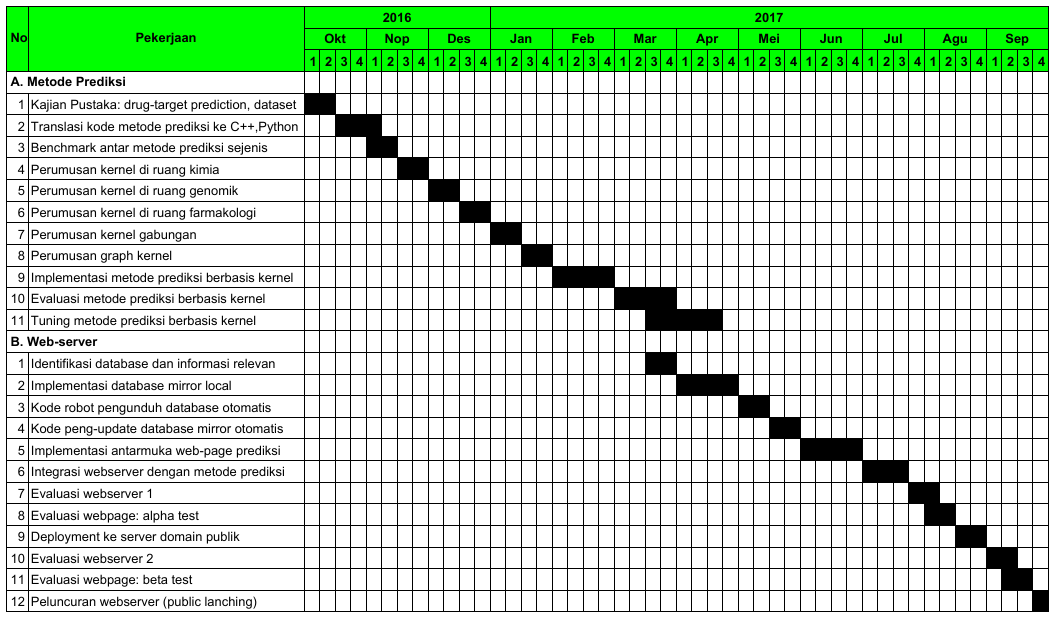
\includegraphics[scale=0.8, angle=0]{pics/timeline.png}
	% 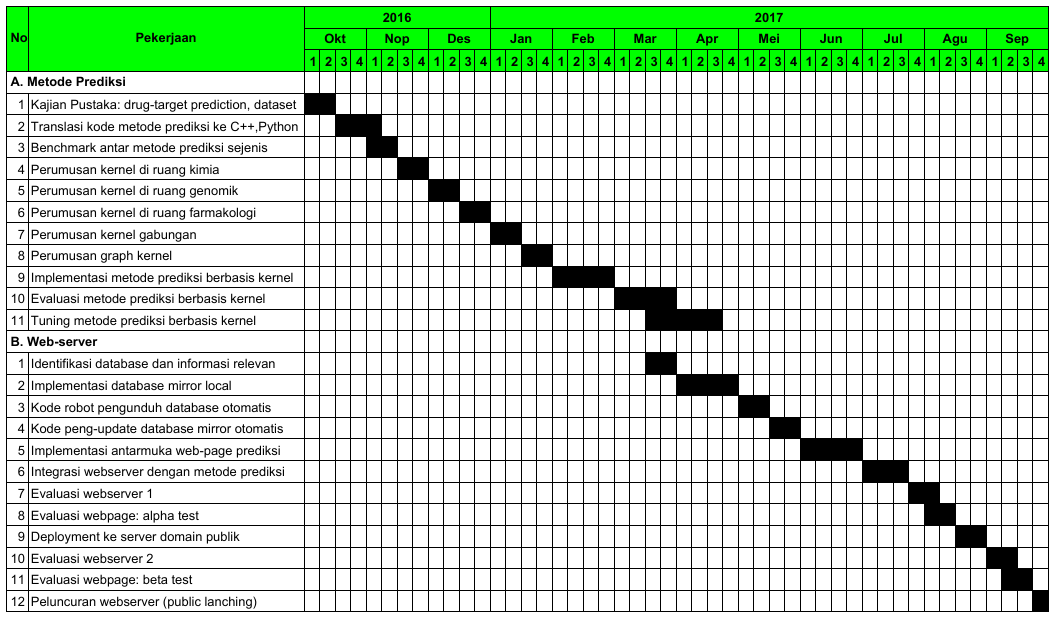
\includegraphics[width=\columnwidth]{pics/timeline.png}
 	\caption{Jadwal pelaksanaan penelitian dalam kurun waktu 12 bulan.}
  	\label{fig:timeline}
\end{figure}  
\end{landscape}
